\documentclass{article}
\usepackage{ifxetex}
\ifxetex
  \usepackage{fontspec}
\else
  \usepackage[T1]{fontenc}
  \usepackage[utf8]{inputenc}
  \usepackage{lmodern}
  \usepackage{float}
  \usepackage{amsmath}
  \usepackage{graphicx}
  \usepackage{morefloats}
  \usepackage{wrapfig}
  \usepackage[top=1in, bottom=1.25in, left=1.1in, right=1.1in]{geometry}
  \usepackage[dvipsnames]{xcolor}
  \usepackage{enumerate}
\fi

\begin{document}
\begin{titlepage}
\begin{center}
    \vspace*{-1in}
    \begin{figure}[htb]
    \begin{center}
    
\includegraphics[width=8cm]{escudo-gde-trans.png}
    \end{center}
\end{figure}
\begin{center}
LICENCIATURA EN FÍSICA \\
\vspace*{0.15in}
DEPARTAMENTO DE FÍSICA \\
\vspace*{0.6in}
\begin{large}
FÍSICA COMPUTACIONAL 1 \\
\end{large}
\vspace*{0.2in}
\rule{80mm}{0.1mm}\\
\vspace*{0.1in}
\begin{large}
\textbf{Reporte 8\\ }
\end{large}
\vspace*{0.3in}
\begin{large}
Alumna: \\
\vspace*{0.1in}
Brambilla Zamorano Fátima Fernanda\\
\end{large}
\vspace*{0.3in}
\rule{80mm}{0.1mm}\\
\vspace*{0.1in}
\begin{large}
Fecha: \\ 16/04/18\\
\end{large}
\end{center}
\end{center}
\end{titlepage}

\section {Introducción y Antecedentes}
Para la octava sesión de Física Computacional 1, trabajamos con el modelo de Van de Pol, el cual es un modelo para un sistema oscilador con amortiguamiento no lineal, el cual explicaremos más adelante, después de mencionar algunos datos sobre los antecedentes del mismo. \\
Balthasar Van der Pol fue un físico neerlandés, cuyos campos de investigación fueron la propagación de ondas, teoría de circuitos y física matemática, y su descubrimiento del oscilador que lleva su nombre le valió para recibir la medalla de honor del \textit{Institute of Radio Engineers}.
La ecuación de Van der Pol es uno de los primeros descubrimientos de la \textit{Teoría del caos}, y esta a su vez tiene una larga historia en la física y la biología, sin embargo, no haremos mención de esta en este documento.

\section {Modelo de Van de Pol}
El oscilador de Van der Pol, es uno con amortiguamiento no lineal, y obedece a la siguiente ecuación de segundo orden:
\begin{equation}
\ddot x -\mu (1-x^2) \dot x +x = 0
\end{equation}
De donde, x es la posición en el tiempo, t es la función del tiempo, y $\mu$ es el amortiguamiento

\section {Exploración de las soluciones del modelo en el Espacio Fase}
En esta sección se presentará como se obtuvieron las gráficas correspondientes a la actividad, y estas mismas para su posterior discusión.
Al igual que en las dos actividades anteriores, se definió un vector al principio del todo,con el cual estaríamos trabajando a lo largo de la actividad, dicho vector almacena el sistema de ecuaciones diferenciales. Se crearon varios tiempos dentro de un intervalo dado, también se definieron las condiciones iniciales y por último se resolvía el sistema de ecuaciones por medio de la función de \textit{odeint}.
\begin{figure}[H]
    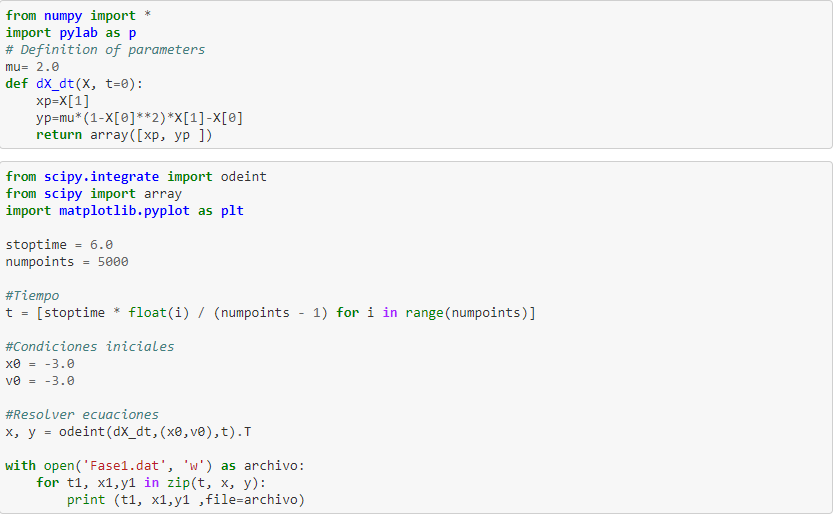
\includegraphics[width=1\textwidth]{Celda1.PNG}
    \centering
    \label{Cod}
\end{figure}
En la imagen de arriba, se pueden ver dos celdas del código, en la primera se muestra la manera en que se definió el vector que se usaría a lo largo de la actividad, mientras que en la segunda se puede ver como empieza a definirse un "campo vectorial" donde se definirá la primera representación gráfica que estamos buscando. Cabe mencionar, que para esta primera gráfica son necesarios cuatro archivos de datos, con los cuales se representaran cuatro fases con diferentes condiciones iniciales. En la segunda celda de la imagen previamente mostrada se pueden ver los datos para el primer archivo de datos.
Como en actividades anteriores, lo que hicimos fue hacer un gráfico de posición contra velocidad, con la diferencia de que en este caso se puede ver el campo vectorial, y la dirección de cada punto, la cual esta dada por la derivada del mismo. Mediante la siguiente sección de código, se hizo una cuadricula que guardaría los valores de la posición y el tiempo, con sus derivadas respectivas.
\begin{figure}[H]
    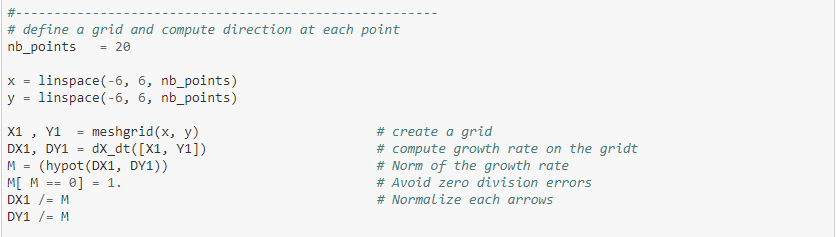
\includegraphics[width=1\textwidth]{Celda2.PNG}
    \centering
    \label{Cod}
\end{figure}
Y la gráfica que se obtuvo es la siguiente:
\begin{figure}[H]
    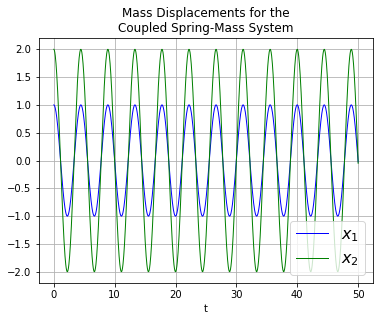
\includegraphics[width=0.5\textwidth]{Grafica1.png}
    \centering
    \label{Cod}
\end{figure}
Para la siguiente gráfica se crearon diferentes archivos de datos con coeficientes de amortiguamiento distintos, y el siguiente gráfico fue la imagen obtenida:
\begin{figure}[H]
    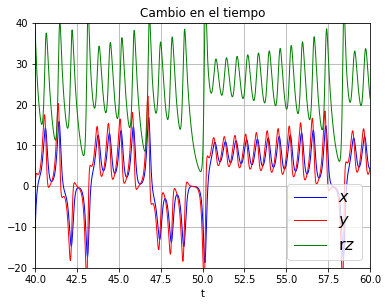
\includegraphics[width=0.5\textwidth]{Grafica2.png}
    \centering
    \label{Cod}
\end{figure}
La siguiente imagen es la representación gráfica del movimiento de un oscilador con una constante de amortiguamiento aproximada a cinco.
\begin{figure}[H]
    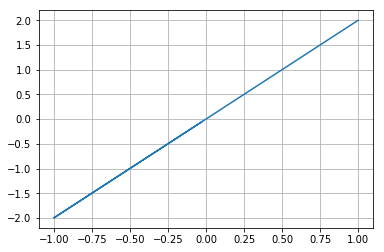
\includegraphics[width=0.5\textwidth]{Grafica3.png}
    \centering
    \label{Cod}
\end{figure}
Por último, se hizo una gráfica con ciertos valores para la amplitud, la constante de amortiguamiento, y la frecuencia. Al vector previamente definido se le agregaron estos tres datos, y se volvió a gráficar la posición contra el tiempo.
\begin{figure}[H]
    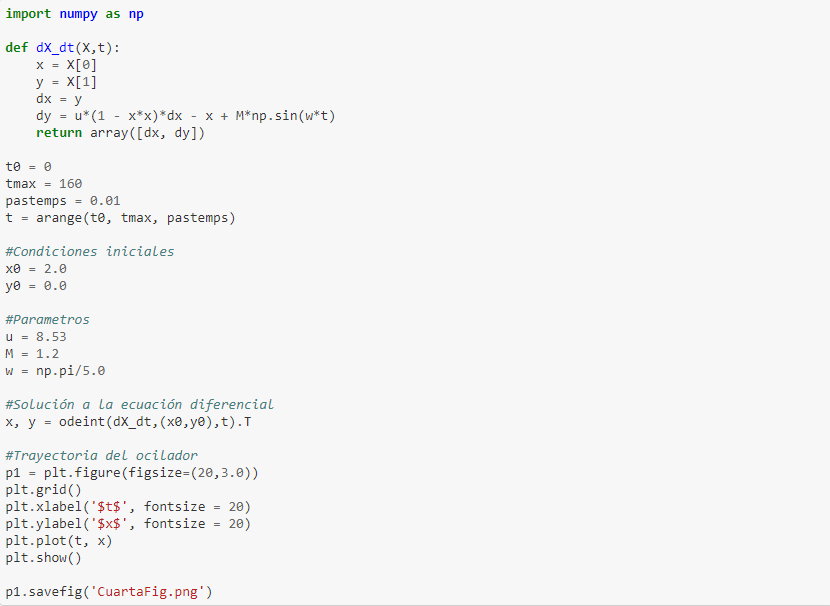
\includegraphics[width=1\textwidth]{Celda3.PNG}
    \centering
    \label{Cod}
\end{figure}
Y se obtuvo la siguiente gráfica:
\begin{figure}[H]
    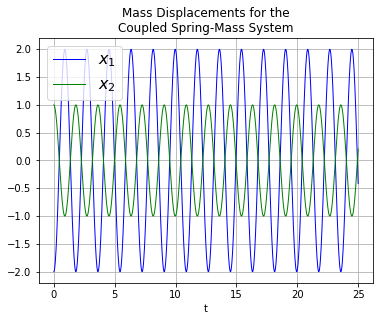
\includegraphics[width=0.5\textwidth]{Grafica4.png}
    \centering
    \label{Cod}
\end{figure}

\section {Resultados y Discusión}
Después de realizar y analizar las gráficas de la actividad, se pudo ver que hay ciertos detalles en cada una de ellas. En primer lugar, la gráfica en la que se hizo uso de un campo vectorial, se puede apreciar que, si bien cada archivo que se uso tenía datos de valor inicial distintos, si el oscilador tiene una sola constante de amortiguamiento, todos llevaran a un mismo ciclo limite de manera eventual, el momento en que lo hagan puede variar, pero terminaran llegando a ese limite. Otra cosa que se puede observar, es que los puntos alejados al ciclo solo se mueven en las direcciones positivas y negativas de y, es decir, no se mueven en el eje x, y entre más se acercan los puntos al limite, empiezan a seguir una curva.
De la segunda gráfica podemos observar la evolución del ciclo limite para valores distintos de la constante de amortiguamiento, siendo visible como el limite se estira cada vez que el valor del amortiguamiento aumenta.
De las gráficas 3 y 4, que nos muestran la posición contra el tiempo de un oscilador forzado, y otro que no, respectivamente, si se comparan, se puede ver que el oscilador forzado tiene cambios bastantes bruscos en su comportamiento, mientras que el oscilador que no lo esta, tiene un comportamiento más periódico.

\section {Conclusiones del Estudio}
El estudiar este tipo de problema nos permite ver como detalles tan pequeños como lo puede ser una fuerza de dispersión, permite encontrar grandes cambios en un sistema, lo que leva a descubrir y analizar nueva información, como lo fue en el caso de Van der Pol.
El estudiar este tipo de problemas con herramientas como Python y Jupyter, hace que examinar la información sea más sencillo, y no solo eso, sino que hace posible encontrar nueva información a partir de distintos tipos de representaciones gráficas, y soluciones númericas a las que antes o no se tenía acceso, o tomaban demasiado tiempo para resolver.
 
\section {Bibliografía}
\begin{itemize}
\item Kanamaru, T. (16 de Enero de 2014). Scholarpedia. \\ Obtenido de \$http://www.scholarpedia.org/article/Van_der_Pol_oscillator$

\item Wikipedia. (05 de Marzo de 2018). Obtenido de \\ \$https://en.wikipedia.org/wiki/Van_der_Pol_oscillator$

\end{itemize}

\section {Ápendice}
    \begin{itemize}
    \item Este ejercicio pareciera simular al desarrollado en las actividades 6 y 7, ¿Qué aprendiste nuevo? \\ En esta actividad se utilizarón gráficos distintos a los que habíamos estado haciendo con anterioridad, de modo que puedo decir que he aprendido a hacer otros tipos de gráficos durante esta actividad, aunque me costo bastante entenderla.
    \item ¿Qué fue lo que más te llamo la atención del oscilador de Van de Pol? \\ No hay algo que haya capturado más mi atención que otra cosa, pienso que todo el tema es bastante interesante.
    \item Has escuchado ya hablar del caos. ¿Por qué sería importante estudiar este oscilador? \\ Creo que es importante estudiar este oscilador, y otros tipos de problemas de la misma naturaleza, ya que son los que más se aproximan a la realidad, puesto que en su mayoría durante los cursos que hemos tomado hasta el momento, se han trabajado problemas en situaciones ideales, es decir, sin tomar en cuenta cosas como la fricción en distintos medios, el movimiento de la tierra en caso de situaciones de movimiento de proyectil, entre otras.
    \item ¿Qué mejorarías en esta actividad? \\ Quizás le haría una introducción a la actividad, explicando como trabajar con ella o con las gráficas que son necesarias generar, ya que fue esto lo que más problema me causo durante la actividad.
    \item Algún comentario adicional antes de dejar de trabajar en Jupyter con Python? \\ Quisiera decir que trabajar en Python por medio de Jupyter ha sido bastante cómodo, aún si en realidad no he entendido del todo todo lo que hemos hecho, al final siento que he aprendido parte de lo necesario para poder manejarlo con más naturalidad de aquí en adelante.
    \item Cerraremos la parte de tu trabajo con Python, ¿Qué te ha parecido? \\ Ha sido una grata experiencia, excepto en la evaluación pasada, y posbilemente en la siguiente.
    \end{itemize}


\end{document}
